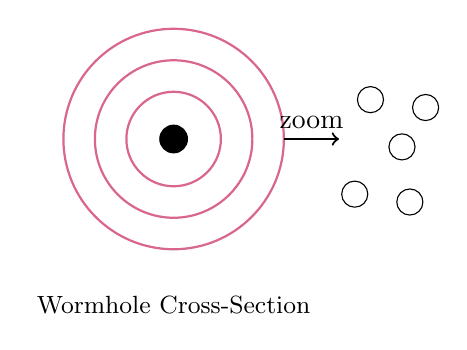
\begin{tikzpicture}[
    macro/.style={circle, draw=black, fill=black, minimum size=10pt},
    ring/.style={circle, draw=purple!60, thick},
    smallnode/.style={circle, draw=black, fill=white, minimum size=5pt},
]

\node[macro] at (0,0) {};

\foreach \r in {0.6,1.0,1.4}{
  \draw[ring] (0,0) circle (\r);
}

\node[smallnode] at (2.5,0.5) {};
\node[smallnode] at (2.9,-0.1) {};
\node[smallnode] at (2.3,-0.7) {};
\node[smallnode] at (3.2,0.4) {};
\node[smallnode] at (3.0,-0.8) {};

\draw[thick, ->] (1.4,0) -- (2.1,0) node[midway, above]{zoom};

\node at (0,-2.1) {\small Wormhole Cross-Section};

\end{tikzpicture}